\documentclass{article}

\usepackage[utf8]{inputenc}
\usepackage[T1]{fontenc}
\usepackage[margin=1in]{geometry}
\usepackage{amsmath,amssymb,amsthm,bm}
\usepackage{graphicx}
\usepackage{booktabs}
\usepackage{caption}
\usepackage{subcaption}
\usepackage{float}
\usepackage{hyperref}
\usepackage[numbers,sort&compress]{natbib}
\usepackage{xcolor}
\usepackage{lmodern}
\usepackage{microtype}
\setlength{\emergencystretch}{2.5em}
\setlength{\textfloatsep}{6pt plus 2pt minus 2pt}
\setlength{\intextsep}{6pt plus 2pt minus 2pt}
\setlength{\abovecaptionskip}{3pt}
\setlength{\belowcaptionskip}{2pt}
\setlength{\floatsep}{6pt plus 2pt minus 2pt}
\hypersetup{colorlinks=true, linkcolor=blue!60!black, citecolor=blue!60!black, urlcolor=blue!70!black}

\graphicspath{{figures/}}

% Reference macros (per writing-guideline: define macros for Eq./Fig./Tab./Sec.
% references so the style can be changed in one place).
\newcommand{\eqnref}[1]{Eq.~\eqref{#1}}
\newcommand{\figref}[1]{Figure~\ref{#1}}
\newcommand{\tabref}[1]{Table~\ref{#1}}
\newcommand{\secref}[1]{Section~\ref{#1}}

\title{Safe Proximal Policy Optimization for Sparse-Reward Classic Control: \\
A PPO-Lagrangian Study on \texttt{MountainCar}}
\author{Hadis Amin\,(u8050066) \quad Muhammad Rafif\,(u7964962) \\[2pt]
Edwar Budiman\,(u7898974) \quad Mukhit Onalbekov\,(u7812910)}
\date{}

\begin{document}
\maketitle

\begin{abstract}
We study constrained RL in \texttt{MountainCar-v0}, building three agents of increasing capability: DQN, PPO, and \emph{Safe~PPO}, a dual-critic PPO-Lagrangian agent with a soft proportional speed constraint. Shared reward shaping isolates the safety mechanism. A two-stage study screens six PPO bases, then sweeps safety hyperparameters on the top three (18 constrained configs, three seeds). The best Safe~PPO matches unconstrained PPO return ($47.3 \pm 0.3$ vs $47.8$) while meeting the budget. Our central finding is compute-qualified: under the fixed 150-epoch protocol, base \emph{cost} (not return) predicts feasibility and the equal-return high-cost base P4 fails every setting --- but repeating P4 for 300 epochs makes 5/6 configs pass at full return, so P4 was undertrained, not intrinsically infeasible. The multiplier $\lambda$ tracks violation magnitude as an interpretable safety regulator. Code, configs, and videos are released.
\end{abstract}


\section{Introduction}
\label{sec:intro}

Reinforcement learning (RL) has produced impressive empirical results across games and control~\citep{mnih2015dqn,schulman2017ppo}, but standard RL implicitly assumes that the agent is free to
maximize reward irrespective of side effects. Many practical applications --- robotics, autonomous
driving, healthcare --- require the agent to satisfy additional safety or operational
constraints. Constrained Markov Decision Processes (CMDPs)~\citep{altman1999cmdp} formalize this
setting by decorating each transition with a scalar \emph{cost} signal, and asking the agent to
maximize return subject to a constraint on expected cumulative cost.

Despite a rich body of constrained-RL work~\citep{achiam2017cpo,ray2019benchmarking,stooke2020responsive,tessler2018reward,chow2018risk},
the classic control benchmark \texttt{MountainCar-v0}~\citep{moore1990mountaincar,brockman2016openaigym}
is rarely used to study safety, because its dynamics are too simple and its reward is too sparse
to make exploration interesting. We argue that exactly these properties make it a useful
\emph{didactic} testbed: the algorithmic interactions between sparse reward, reward shaping, and
constraint enforcement become visible without confounding effects from large neural networks or
visual inputs.

\paragraph{Contributions.}
\begin{enumerate}
    \item Three progressively complex agents (DQN, PPO, Safe~PPO) on a shared energy-shaped \texttt{MountainCar} environment, with matched hyperparameters to isolate the safety mechanism.
    \item A soft \emph{proportional} speed cost that produces a smooth signal, keeping the PPO-Lagrangian update well-behaved under sparse reward.
    \item A \emph{dual-critic} Safe~PPO with log-parameterized $\lambda$ updated by dual ascent; the best config matches unconstrained return while satisfying the budget.
    \item A \emph{two-stage} protocol showing that base unconstrained cost --- not return --- predicts constrained feasibility under a fixed training budget; a longer P4 rerun separates this compute effect from intrinsic feasibility.
    \item A modular codebase with reproducible configs, automated stage runners, training videos, and multi-seed scripts.
\end{enumerate}


\section{Related Work}
\label{sec:related}

\paragraph{Deep value methods.} DQN~\citep{mnih2015dqn} popularized value-based deep RL via a
replay buffer and a slow-moving target network, both of which we re-use in our Phase~1 baseline.

\paragraph{Policy gradient methods.} PPO~\citep{schulman2017ppo} introduces a clipped surrogate
objective that bounds the size of each policy update; combined with Generalized Advantage
Estimation~\citep{schulman2016gae} it is the de-facto on-policy baseline in continuous and
discrete control.

\paragraph{Constrained / safe RL.} CMDPs~\citep{altman1999cmdp} are the standard framework for
constrained sequential decision making. CPO~\citep{achiam2017cpo} performs a constrained policy
update via a trust region. Reward-constrained Policy Optimization~\citep{tessler2018reward} and
the PPO-Lagrangian baseline of \citet{ray2019benchmarking} adapt a Lagrangian multiplier via
dual ascent --- the family our Safe~PPO belongs to. PID-Lagrangian~\citep{stooke2020responsive}
further stabilizes the multiplier with proportional/integral/derivative control. We deliberately
use the simpler dual-ascent variant because it surfaces the multiplier dynamics most clearly.

\paragraph{Reward shaping.} Potential-based reward shaping~\citep{ng1999rewardshaping} adds
$\gamma\Phi(s')-\Phi(s)$ and provably preserves the optimal policy. Our height bonus is a
\emph{non}-potential, mechanical-energy-style term added directly to the reward: it accelerates
learning under sparse reward but does modify the objective, so all agents optimize the same
shaped return and our comparisons are internally consistent rather than policy-invariant.


\section{Background}
\label{sec:background}

\subsection{Markov Decision Processes}
A discounted MDP is a tuple $\mathcal{M} = (\mathcal{S}, \mathcal{A}, P, R, \gamma)$ with
states $\mathcal{S}$, actions $\mathcal{A}$, transition kernel $P$, reward $R$, and discount
$\gamma \in [0,1)$. The agent seeks a policy $\pi$ maximizing
$J_R(\pi) = \mathbb{E}_{\pi}\!\left[\sum_{t=0}^{\infty} \gamma^t R(s_t, a_t)\right]$.

\subsection{Constrained MDPs}
A CMDP~\citep{altman1999cmdp} augments an MDP with a non-negative cost $C(s,a) \ge 0$ and a
budget~$d$. The constrained problem is
\begin{equation}
\label{eq:cmdp}
\max_{\pi}\ J_R(\pi) \quad \text{subject to} \quad
J_C(\pi) := \mathbb{E}_{\pi}\!\left[\sum_{t=0}^{\infty} \gamma^t C(s_t, a_t)\right] \le d.
\end{equation}
The Lagrangian relaxation introduces $\lambda \ge 0$ and yields the saddle-point problem
$\max_\pi \min_{\lambda \ge 0}\ J_R(\pi) - \lambda \bigl(J_C(\pi) - d\bigr)$.

\subsection{PPO Clipped Surrogate Objective}
For a stochastic policy $\pi_\theta$ with old parameters $\theta_{\text{old}}$, PPO maximizes
\begin{equation}
\label{eq:ppo}
L^{\text{CLIP}}(\theta) = \mathbb{E}_t\!\left[
\min\!\Bigl( r_t(\theta)\,\hat{A}_t,\ \mathrm{clip}\bigl(r_t(\theta), 1-\epsilon, 1+\epsilon\bigr)\,\hat{A}_t \Bigr)
\right],
\end{equation}
where $r_t(\theta) = \pi_\theta(a_t\!\mid\!s_t) / \pi_{\theta_{\text{old}}}(a_t\!\mid\!s_t)$ and
$\hat{A}_t$ is the GAE advantage~\citep{schulman2016gae}. In practice both PPO and Safe~PPO add
the same entropy bonus $\beta\,\mathcal{H}[\pi_\theta]$ to this objective to encourage
exploration~\citep{mnih2016a3c}.


\section{Method: Safe~PPO with Dual-Critic and Adaptive $\lambda$}
\label{sec:method}

\subsection{Constrained \texttt{MountainCar}}
We instantiate the CMDP via two wrappers around \texttt{MountainCar-v0}:
\textsc{ShapedMountainCar} adds a height-based shaping bonus
$\phi(s) = 1.5 \cdot |x - (-0.5)|$ directly to the reward (not potential-based in the sense of
\citet{ng1999rewardshaping}: it modifies the objective, but identically for every agent) and a
$+100$ completion bonus on termination;
\textsc{ConstrainedMountainCar} additionally emits a proportional safety cost
\begin{equation}
\label{eq:cost}
C(s, a) = \max\!\bigl(0,\ 100\,(|\dot{x}| - v_{\max})\bigr), \quad v_{\max} = 0.04.
\end{equation}
The proportional form gives a smooth, informative signal: speeding by twice the margin yields
twice the cost. We justify the specific values $v_{\max}{=}0.04$ and $d{=}15$ with a feasibility probe in \secref{sec:setup} (\figref{fig:probe}).

\subsection{Dual-critic architecture}
Safe~PPO uses three MLP heads sharing the same input but with separate weights:
an actor producing categorical logits, a reward critic $V_R(s)$, and a cost critic $V_C(s)$.
For both reward and cost streams we compute Generalized Advantage Estimation~\citep{schulman2016gae} with discount $\gamma{=}0.99$ and $\lambda_{\text{GAE}}{=}0.95$.
The reward advantage $\hat{A}_t^R$ is mean-centered and unit-scaled; the cost advantage
$\hat{A}_t^C$ is only \emph{scaled}, not centered, so that its sign continues to indicate
whether an action is safer or less safe than the average. Crucially, this scaling is applied
only when the batch contains non-zero cost: when no violation has occurred we set
$\hat{A}_t^C{=}0$ rather than normalizing critic noise, so that Safe~PPO reduces exactly to PPO
until a genuine constraint signal appears (see \secref{sec:discussion}).

\subsection{Policy update}
With clip parameter $\epsilon = 0.2$, the policy maximizes the Lagrangian-augmented surrogate
\begin{equation}
\label{eq:safeppo}
L(\theta) =
\underbrace{\mathbb{E}_t\!\left[ \min\bigl(r_t(\theta)\hat{A}^R_t, \mathrm{clip}(r_t(\theta), 1\!-\!\epsilon, 1\!+\!\epsilon)\hat{A}^R_t\bigr)\right]}_{\text{reward objective}}
\;-\;
\lambda \cdot
\underbrace{\mathbb{E}_t\!\left[ r_t(\theta)\,\hat{A}^C_t \right]}_{\text{cost objective}}
\;+\; \beta\,\mathcal{H}[\pi_\theta],
\end{equation}
with entropy bonus $\beta{=}0.01$~\citep{mnih2016a3c}. The reward branch uses the PPO clip; the cost branch uses an
unclipped surrogate, in line with PPO-Lagrangian baselines~\citep{ray2019benchmarking}.

\subsection{Adaptive Lagrangian multiplier}
We parameterize $\lambda = \exp(\ell)$ with unconstrained $\ell \in \mathbb{R}$. After each
policy/critic update we run one Adam step on
\begin{equation}
\label{eq:lambdaupdate}
\mathcal{L}_\lambda(\ell) = -\exp(\ell)\,\bigl(\hat{J}_C - d\bigr),
\end{equation}
where $\hat{J}_C$ is the empirical mean of the cost-return targets in the current batch.
Note that $\hat{J}_C$ is the mean \emph{discounted} cost-return of \eqnref{eq:lambdaupdate}; in the undiscounted episode units used in our figures this corresponds to a budget ${\approx}d/0.52$.
This yields the dual-ascent update $\ell \leftarrow \ell + \alpha_\lambda \exp(\ell)(\hat{J}_C - d)$,
which monotonically increases $\lambda$ when the constraint is violated and shrinks it otherwise.
The initialization $\ell_0$ and step size $\alpha_\lambda$ are tuned in Stage~2 (\secref{sec:setup}).

Algorithm~1 summarizes the full procedure.

\begin{figure}[H]
\centering
\begin{minipage}{0.95\linewidth}
\hrule\medskip
\textbf{Algorithm 1: Safe~PPO with dual critics and adaptive $\lambda$}
\medskip\hrule\medskip
\textbf{Initialize} actor $\pi_\theta$, reward critic $V_R$, cost critic $V_C$, multiplier $\ell$ \\[2pt]
\textbf{For} epoch $k = 1 \ldots K$ \textbf{do} \\
\hspace*{1em} 1.\ Collect $T$ steps in \textsc{ConstrainedMountainCar}, storing $(s_t, a_t, r_t, c_t, V_R, V_C, \log\pi)$ \\
\hspace*{1em} 2.\ Compute $\hat{A}^R, \hat{A}^C$ via dual GAE; targets $\hat{R}^R, \hat{R}^C$ \\
\hspace*{1em} 3.\ Normalize $\hat{A}^R$ (mean/std); scale $\hat{A}^C$ by std only \emph{if} batch cost ${>}0$, else $\hat{A}^C \gets 0$ \\
\hspace*{1em} 4.\ \textbf{For} $i = 1 \ldots N_\pi$ \textbf{do} update $\theta$ via Adam on $-L(\theta)$ in \eqnref{eq:safeppo} \\
\hspace*{1em} 5.\ \textbf{For} $i = 1 \ldots N_V$ \textbf{do} update $V_R, V_C$ via MSE on $\hat{R}^R, \hat{R}^C$ \\
\hspace*{1em} 6.\ $\hat{J}_C \gets \mathrm{mean}(\hat{R}^C)$;\ \  $\ell \gets \ell + \alpha_\lambda \exp(\ell)(\hat{J}_C - d)$ \\
\textbf{End for}
\medskip\hrule
\end{minipage}
\end{figure}


\section{Experimental Setup}
\label{sec:setup}

\textbf{Environment.} \texttt{MountainCar-v0}~\citep{brockman2016openaigym} with maximum episode
length 200 and reward $-1$ per step. We wrap with \textsc{ShapedMountainCar} for DQN/PPO and
\textsc{ConstrainedMountainCar} ($v_{\max}{=}0.04$, $d{=}15$) for Safe~PPO.

\textbf{Constraint design.} $v_{\max}$ and $d$ are fixed by a \emph{feasibility probe} (\figref{fig:probe}): a hand-coded speed-capped controller swept over 200 random starts. $v_{\max}{=}0.04$ is the tightest cap with 100\% solve rate (at $0.035$ solve rate falls to $70\%$); it is also the cost threshold, so it defines the floor of achievable cost. The thriftiest $100\%$-solving run costs $\approx 11$ (worst case $\approx 16$); plain speeding costs $\approx 29$. Setting $d{=}15$ places the budget tight but above the achievable floor --- feasible by construction.

\begin{figure}[H]
  \centering
  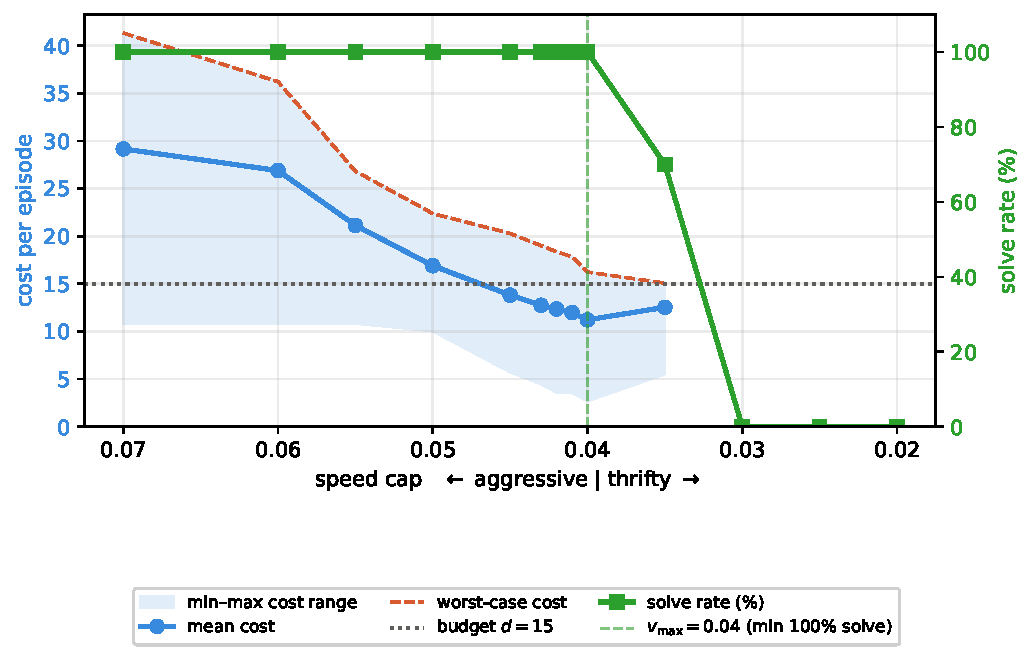
\includegraphics[width=0.44\linewidth]{fig7_feasibility_probe.pdf}
  \caption{Feasibility probe (no learning): episode cost and solve rate versus speed cap for a
  hand-coded capped controller over 200 random starts. Cost falls as the cap tightens, but below
  $v_{\max}{=}0.04$ (green dashed line) the solve rate drops below $100\%$. The thriftiest solving
  cap averages cost $\approx 11$, against the budget $d{=}15$ (dotted) and the $\approx 29$ of
  unconstrained speeding, so the constraint is tight but feasible.}
  \label{fig:probe}
\end{figure}

\textbf{Networks.} Two-layer MLPs with hidden size 64. DQN uses ReLU; PPO/Safe~PPO use Tanh.

\textbf{Optimizers.} Adam everywhere. DQN: lr $10^{-3}$, batch 64, target sync every five episodes,
$\epsilon$-greedy with decay 0.995 and floor 0.05. PPO / Safe~PPO: $V$-lr $10^{-3}$, 80 policy and
80 critic iterations per epoch, clip $\epsilon{=}0.2$, GAE $\gamma{=}0.99$, $\lambda{=}0.95$,
4000 environment steps per epoch. The policy learning rate and entropy bonus are \emph{tuned} in
Stage~1 (below) rather than fixed.

\textbf{Two-stage protocol.} \emph{Stage~1} screens six PPO bases ($\text{lr} \in \{1,3,10\}\!\times\!10^{-4}$, $\beta \in \{0, 0.01\}$, configs P1--P6) over three seeds. Bases are ranked by $\text{mean}-\text{std}$ of return, keeping only those with $\ge 50\%$ solve rate; the top three (P6, P5, P4) advance. A passive cost (computed with \eqnref{eq:cost} but never optimized) is logged as a feasibility indicator. \emph{Stage~2} sweeps $\alpha_\lambda \in \{0.02, 0.03, 0.05\}$ and $\ell_0 \in \{-1, 0\}$ on each base (S1--S18, $d{=}15$, three seeds). A config \emph{passes} if cost $\le 15$ and no seed collapses (return drops $>30\%$ without recovering in the last 20 epochs).

\textbf{Winning configuration.} The selected Safe~PPO (S6) uses base P6 ($\pi$-lr $10^{-3}$,
$\beta{=}0.01$) with $\alpha_\lambda = 0.05$ and $\ell_0 = 0$ ($\lambda_0 = 1$), $d=15$.

\textbf{Budgets.} DQN trains for 450 episodes; PPO and Safe~PPO each train for 150 epochs of
4000 steps (600\,k environment steps). Stage~1 is $6\times 3 = 18$ runs; Stage~2 is
$18 \times 3 = 54$ runs.

\textbf{Reproducibility.} Python, NumPy, and PyTorch are seeded from a single integer. Stages run via \texttt{run\_stage1} / \texttt{run\_stage2} scripts; metrics go to \texttt{results/<config>/seed\_<s>/metrics.json}.

\textbf{Compute.} RTX~5050 (8\,GB); $\approx280$\,s per run. Stage~1 (18 runs): 1\,h\,24\,m; Stage~2 (54 runs): 4\,h\,12\,m; total $\approx5.6$\,h.


\section{Results}
\label{sec:results}

\subsection{Stage 1: base selection}
\tabref{tab:stage1} and \figref{fig:stage1} report the six unconstrained PPO bases.
The learning rate dominates: at $10^{-4}$ (P1, P2) the policy never solves within 150 epochs
(0\% solved, return $\approx -150$); at $3\!\times\!10^{-4}$ without entropy (P3) learning is
unstable across seeds (65\% solved, return $-29.2 \pm 92.8$); and at $\{3\!\times\!10^{-4},
10^{-3}\}$ with entropy (P4--P6) the agent solves on every seed with return $\approx 47.5$.
Crucially, among the three \emph{solving} bases the passive speeding cost differs almost
two-fold: P4 reaches return $47.5$ at cost $28.9$, whereas P5 and P6 reach the same return at
cost $\approx 15$. Because return alone cannot distinguish them, this cost gap --- invisible to
the PPO objective --- is exactly the information needed to anticipate Stage~2 feasibility.

\begin{table}[H]
  \centering
  \caption{Stage 1 (unconstrained PPO) base screening. Final-window (last ten epochs) mean$\pm$std
  over three seeds. ``Avg cost'' is logged passively (not optimized). Score $=
  \text{mean}-\text{std}$ of return; the top-three solving bases are carried into Stage~2.}
  \label{tab:stage1}
  \begin{tabular}{lccccccc}
    \toprule
    ID & lr & $\beta$ & Return & Avg cost & Solved & Score & Top-3 \\
    \midrule
    P1 & $10^{-4}$ & 0    & $-149.7 \pm 7.3$  & $0.0$  & 0\%   & $-157.1$ & \\
    P2 & $10^{-4}$ & 0.01 & $-145.8 \pm 0.2$  & $0.0$  & 0\%   & $-146.0$ & \\
    P3 & $3\!\times\!10^{-4}$ & 0    & $-29.2 \pm 92.8$  & $24.2$ & 65\%  & $-122.0$ & \\
    P4 & $3\!\times\!10^{-4}$ & 0.01 & $47.5 \pm 1.1$    & $28.9$ & 100\% & $46.4$   & \checkmark \\
    P5 & $10^{-3}$ & 0    & $47.8 \pm 1.4$    & $15.2$ & 100\% & $46.4$   & \checkmark \\
    P6 & $10^{-3}$ & 0.01 & $47.8 \pm 0.2$    & $15.0$ & 100\% & $\mathbf{47.6}$   & \checkmark \\
    \bottomrule
  \end{tabular}
\end{table}

\begin{figure}[t]
  \centering
  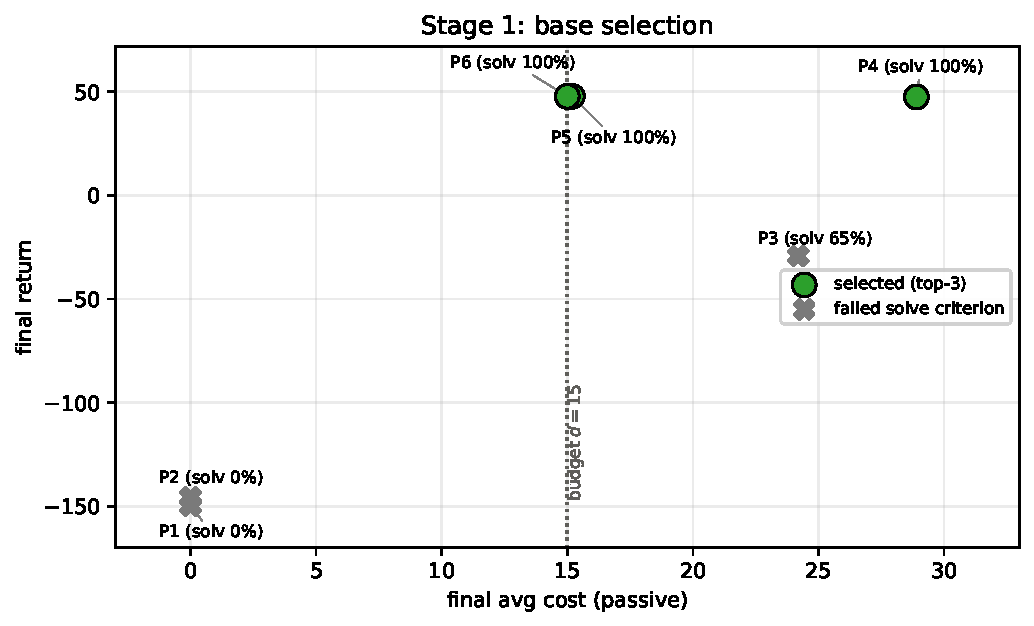
\includegraphics[width=0.43\linewidth]{fig4_stage1_selection.pdf}
  \caption{Stage 1 base selection: final return vs.\ passive cost (three-seed mean). Green circles are
  the three selected bases; grey crosses fail the solve criterion. The three solving bases
  (P4, P5, P6) share the same return but split sharply by cost, with P4 sitting nearly twice as
  far past the budget line as P5/P6.}
  \label{fig:stage1}
\end{figure}

\subsection{Stage 2: safety sweep and the role of the base}
\tabref{tab:stage2} and \figref{fig:stage2} show all 18 constrained configurations.
\textbf{Every P4-based config fails within the 150-epoch sweep}, clustering at cost $29$--$34$ regardless of $\alpha_\lambda$ or $\ell_0$: a base that overspeeds at cost $\approx 29$ when unconstrained moves too slowly toward the budget under this fixed compute allocation (\secref{sec:discussion}). The P6- and P5-based configs populate the feasible region; three pass: S6 (P6, cost $15.0$, return $47.3$), S4 (P6, cost $14.7$, return $46.8$), and S10 (P5, cost $11.6$, return $40.2 \pm 8.3$). The \emph{base's unconstrained cost}, not its return, governs the fixed-budget sweep outcome --- selecting by return alone (which keeps P4) is actively counterproductive when compute is capped.

A secondary effect is the initial multiplier. Across bases, $\ell_0 = 0$ ($\lambda_0 = 1$) meets
the budget far more often than $\ell_0 = -1$: starting with real constraint pressure pulls cost
down before the policy commits to a fast solution. The one failure mode of an aggressive start is
over-constraint --- S8 (P5, $\alpha_\lambda{=}0.02$, $\ell_0{=}0$) drives cost to $2.7$ but
collapses on one seed ($-27.2 \pm 52.5$). The winner therefore pairs a low-cost base with a warm
multiplier start and the largest sweep $\alpha_\lambda{=}0.05$.

\begin{table}[t]
  \centering
  \caption{Stage 2 (Safe~PPO) sweep. Final-window (last ten epochs) mean$\pm$std over three seeds, with
  $d{=}15$ fixed. \emph{Pass} requires cost $\le 15$ and no seed collapse. S6 (bold) is the winner;
  S8 meets the cost numerically but collapses on one seed. Bases: B1=P6, B2=P5, B3=P4.}
  \label{tab:stage2}
  \begin{tabular}{llcccccc}
    \toprule
    ID & Base & $\alpha_\lambda$ & $\ell_0$ & Avg cost & $\le 15$ & Return & Pass \\
    \midrule
    S1 & P6 & 0.02 & $-1$ & $19.2$ & no  & $46.0 \pm 1.3$ & \\
    S2 & P6 & 0.02 & $0$  & $18.9$ & no  & $29.6 \pm 8.8$ & \\
    S3 & P6 & 0.03 & $-1$ & $16.0$ & no  & $47.9 \pm 0.8$ & \\
    S4 & P6 & 0.03 & $0$  & $14.7$ & yes & $46.8 \pm 0.1$ & \checkmark \\
    S5 & P6 & 0.05 & $-1$ & $22.1$ & no  & $45.6 \pm 2.8$ & \\
    \textbf{S6} & P6 & 0.05 & $0$ & $\mathbf{15.0}$ & yes & $\mathbf{47.3 \pm 0.3}$ & \checkmark \\
    \midrule
    S7  & P5 & 0.02 & $-1$ & $17.1$ & no  & $46.9 \pm 3.5$   & \\
    S8  & P5 & 0.02 & $0$  & $2.7$  & yes & $-27.2 \pm 52.5$ & \\
    S9  & P5 & 0.03 & $-1$ & $17.7$ & no  & $47.8 \pm 1.0$   & \\
    S10 & P5 & 0.03 & $0$  & $11.6$ & yes & $40.2 \pm 8.3$   & \checkmark \\
    S11 & P5 & 0.05 & $-1$ & $17.4$ & no  & $47.5 \pm 1.3$   & \\
    S12 & P5 & 0.05 & $0$  & $16.3$ & no  & $48.1 \pm 0.2$   & \\
    \midrule
    S13 & P4 & 0.02 & $-1$ & $32.1$ & no & $39.4 \pm 7.5$  & \\
    S14 & P4 & 0.02 & $0$  & $33.9$ & no & $32.8 \pm 12.2$ & \\
    S15 & P4 & 0.03 & $-1$ & $31.6$ & no & $36.5 \pm 11.5$ & \\
    S16 & P4 & 0.03 & $0$  & $29.2$ & no & $35.4 \pm 15.8$ & \\
    S17 & P4 & 0.05 & $-1$ & $32.6$ & no & $38.4 \pm 9.8$  & \\
    S18 & P4 & 0.05 & $0$  & $33.5$ & no & $37.3 \pm 10.3$ & \\
    \bottomrule
  \end{tabular}
\end{table}

\begin{figure}[t]
  \centering
  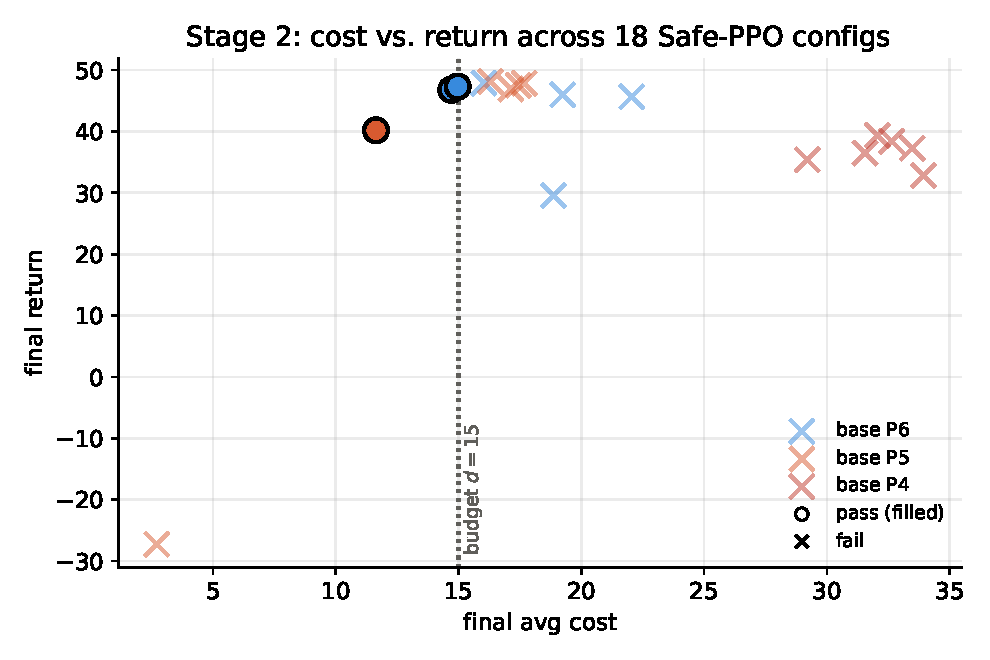
\includegraphics[width=0.47\linewidth]{fig5_stage2_scatter.pdf}
  \caption{Stage 2: final cost vs.\ return for all 18 Safe-PPO configurations (three-seed mean),
  colored by base (P6 blue, P5 green, P4 red). Filled circles pass (cost $\le 15$, no collapse);
  crosses fail. After 150 epochs all P4-based configs sit far past the budget; the feasible passing configs are
  built on the low-cost bases P6 and P5. S8 meets the cost numerically but collapses.}
  \label{fig:stage2}
\end{figure}

\subsection{The winning policy}
\figref{fig:winner} shows the winner's training dynamics. Return rises to $\approx 47$ within the first $\sim 40$ epochs and the safety cost settles at the budget ($15.0$). The multiplier starts at $\lambda_0{=}1$, peaks at $\approx 0.95$ as cost first appears, then relaxes to $\approx 0.09$ once the constraint is met --- the self-regulating behavior of dual ascent, with $\lambda$'s trajectory serving as a running estimate of constraint bindingness.

\begin{figure}[t]
  \centering
  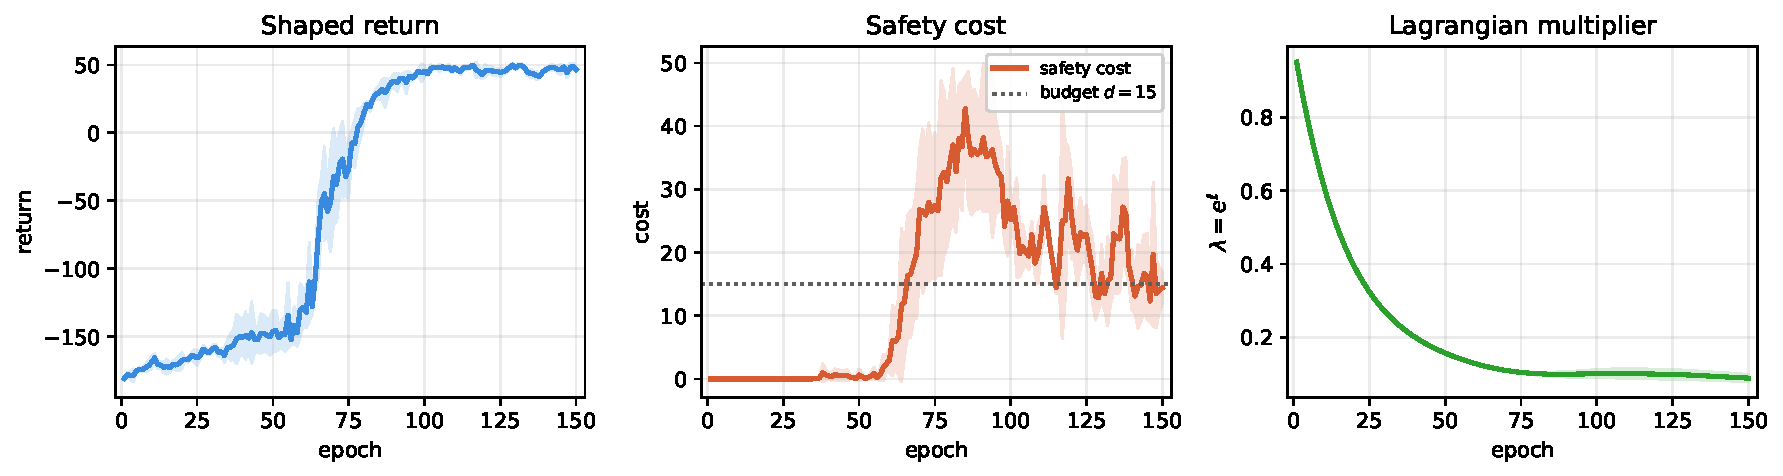
\includegraphics[width=0.72\linewidth]{fig_winner_dynamics.pdf}
  \caption{Winning Safe~PPO (S6) dynamics, three-seed mean$\pm$std: shaped return (left), safety
  cost against the budget $d{=}15$ (middle), and the Lagrangian multiplier $\lambda$ (right). The
  constraint becomes binding early; $\lambda$ peaks then relaxes as cost converges toward the
  budget with no return loss.}
  \label{fig:winner}
\end{figure}

\subsection{Comparison and summary}
\figref{fig:curves} compares the three agents' shaped return as a function of environment
steps. DQN reaches a steady-state return of $\approx 27$; the PPO base and the constrained winner
both converge to $\approx 47$, with Safe~PPO essentially overlapping unconstrained PPO --- the
constraint costs no measurable return on this task. \tabref{tab:final} summarizes final-window
performance.

\begin{figure}[t]
  \centering
  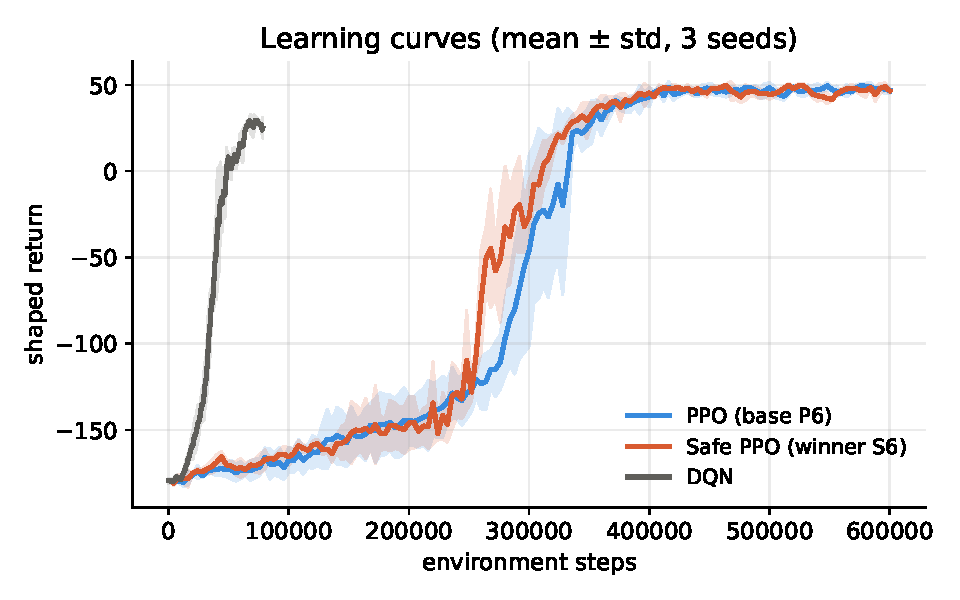
\includegraphics[width=0.45\linewidth]{fig1_learning_curves.pdf}
  \caption{Shaped return vs.\ environment steps for DQN, the PPO base (P6), and the Safe~PPO winner
  (S6). Mean$\pm$std across three seeds. The two PPO variants are nearly indistinguishable.}
  \label{fig:curves}
\end{figure}

\begin{table}[t]
  \centering
  \caption{Final-window performance. Mean$\pm$std across three seeds (\texttt{--seeds 0 1 2}). Final
  return is averaged over the last 50 episodes (DQN) or last ten epochs (PPO, Safe~PPO). PPO is the
  selected base P6; Safe~PPO is the winner S6.}
  \label{tab:final}
  \begin{tabular}{lcccc}
    \toprule
    Algorithm & Final return $\uparrow$ & Final cost $\downarrow$ & $\lambda$ end & Solved \\
    \midrule
    DQN              & $26.8 \pm 2.0$ & --            & --              & $99\%$ \\
    PPO (base P6)    & $\mathbf{47.8 \pm 0.2}$ & $15.0$        & --              & $100\%$ \\
    Safe~PPO (S6)    & $47.3 \pm 0.3$ & $15.0 \le 15$ & $0.09$          & $100\%$ \\
    \bottomrule
  \end{tabular}
\end{table}


\section{Discussion}
\label{sec:discussion}

\paragraph{Why the high-cost base fails at 150 epochs---and what rescues it.}
Every P4 config settles \emph{above} P4's own unconstrained cost ($29$--$34$ vs $28.9$), with $\lambda$ collapsed to ${\approx}0.09$: a horizon/timing failure, not infeasibility. P4 ($\pi$-lr $3\times10^{-4}$) first solves only near epoch~80 and incurs no cost before then, so the dual update decays $\lambda$ through the long zero-cost warmup, leaving too little time to drive cost down. The units of \eqnref{eq:lambdaupdate} sharpen this: P4's cost ($\approx 29$) sits at the effective episode budget $d/0.52 \approx 29$, i.e.\ on the zero-gradient threshold. Repeating the block with the \emph{original} Safe~PPO and the single change $150\!\to\!300$ epochs (\tabref{tab:p4300}) makes 5/6 configs pass at full return; the lone miss (S22, $15.6$) is one high-cost seed. P4 is thus not intrinsically infeasible, and ``base cost decides feasibility'' is best read as a screening rule at \emph{fixed compute}: low-cost bases pass out of the box, high-cost P4 needs a longer horizon (PID-Lagrangian or budget annealing may reduce this).

\begin{table}[H]
  \centering
  \small
  \setlength{\tabcolsep}{5pt}
  \caption{High-cost base P4 at 300 epochs (S19--S24) vs.\ the original 150-epoch runs (S13--S18):
  \emph{original} Safe~PPO, only \texttt{epochs} changed; three-seed mean$\pm$std, $d{=}15$, all solve
  at $1.00$. \emph{Pass} = mean cost $\le 15$. Doubling the horizon turns every P4 config from a budget
  failure into (near-)feasible at full return --- undertraining, not task physics.}
  \label{tab:p4300}
  \begin{tabular}{lcccccc}
    \toprule
    Config & $\alpha_\lambda$ & $\ell_0$ & cost (150) & cost (300) & Return (300) & Pass \\
    \midrule
    S13$\to$S19 & 0.02 & $-1$ & $32.1$ & $13.0 \pm 4.1$ & $48.9 \pm 0.3$ & \checkmark \\
    S14$\to$S20 & 0.02 & $0$  & $33.9$ & $10.8 \pm 3.7$ & $48.3 \pm 1.7$ & \checkmark \\
    S15$\to$S21 & 0.03 & $-1$ & $31.6$ & $11.2 \pm 3.1$ & $49.2 \pm 0.7$ & \checkmark \\
    S16$\to$S22 & 0.03 & $0$  & $29.2$ & $15.6 \pm 7.5$ & $48.4 \pm 0.8$ & \\
    S17$\to$S23 & 0.05 & $-1$ & $32.6$ & $12.4 \pm 4.5$ & $48.5 \pm 0.7$ & \checkmark \\
    S18$\to$S24 & 0.05 & $0$  & $33.5$ & $13.1 \pm 0.3$ & $48.1 \pm 1.1$ & \checkmark \\
    \bottomrule
  \end{tabular}
\end{table}

\paragraph{Sparse reward delays constraint pressure.}
Until reward shaping motivates the agent to reach the flag it rarely hits the speed limit, so the cost critic and multiplier receive almost no signal; dual ascent begins useful work only once reward and cost signals co-activate. Moreover, the height bonus rewards distance from the valley floor and so mildly \emph{encourages} the very speed the cost penalizes; the shaping and the safety constraint are in direct tension, which is part of what makes this CMDP non-trivial.

\paragraph{Cost-advantage normalization in the zero-cost regime.}
When the environment emits no cost, $\hat{A}^C$ is pure critic noise; standardizing it injects $\mathcal{O}(\lambda)$ gradient noise on every update. Setting $\hat{A}^C{=}0$ whenever the batch has no cost lets Safe~PPO reduce exactly to PPO until a genuine violation occurs, restoring exploration without affecting constrained behavior. We recommend this guard for any PPO-Lagrangian on sparse-cost CMDPs.

\paragraph{The initial multiplier is a feasibility knob, with a collapse failure mode.}
A cold start ($\ell_0{=}{-1}$) lets the agent commit to a fast solution before the penalty bites, and most such configs end above the budget; a warm start ($\ell_0{=}0$, $\lambda_0{=}1$) applies early pressure and meets the budget far more often. But S8 (low $\alpha_\lambda$, warm start) drives cost to $2.7$ yet collapses on one seed. The multiplier has a usable but narrow operating band; PID-Lagrangian~\citep{stooke2020responsive} widens it automatically.

\paragraph{Soft budget, met in practice.}
The winner converges to cost $15.0$ at no return cost. The proportional penalty creates a genuine equilibrium rather than a hard projection; feasibility is nonetheless thin ($d{=}15$ sits just above the hand-coded floor of $\approx 11$). A hard-constraint variant (CPO~\citep{achiam2017cpo}) would project onto the feasible set; we leave this to future work.

\paragraph{Limitations.}
(i)~Three seeds; several Stage~2 configs show high variance and warrant a five-seed re-run, and S6 was the only configuration meeting both criteria \emph{under this three-seed protocol} (the S6/S12 cost gap is within seed noise).
(ii)~$\lambda$ is updated against the discounted cost-return while feasibility is checked in undiscounted episode units (\secref{sec:method}).
(iii)~All reported returns and costs are stochastic training-rollout statistics; deterministic (argmax) evaluation is consistently \emph{safer}, so these numbers if anything understate deployment-time safety.
(iv)~\texttt{MountainCar} is two-dimensional; higher-dimensional conclusions require further experiments~\citep{ray2019benchmarking}.


\section{Conclusion}
\label{sec:conclusion}

We compared DQN, PPO, and a dual-critic Safe~PPO on sparse-reward \texttt{MountainCar} via a
two-stage study. The tuned Safe~PPO meets the budget ($15.0 \le 15$) at a return indistinguishable
from the unconstrained base. Under a fixed 150-epoch protocol, constrained feasibility is governed
by a base's unconstrained \emph{cost}, not its return; we further show this is a truncated-horizon
artifact, since repeating the high-cost P4 block for 300 epochs with the same implementation makes
5/6 configs pass and all six solve at full return. Base cost is thus a cheap feasibility screen at
fixed method and compute, and the simple setting keeps the dual-ascent dynamics pedagogically clear.
Future work: five-seed confirmation, PID-Lagrangian and budget annealing to remove the horizon
dependence, hard-constraint comparisons, and higher-dimensional CMDPs.

\vspace{-6pt}
{\scriptsize
\setlength{\bibsep}{0pt}
\bibliographystyle{plainnat}
\bibliography{references}
}

\end{document}
